\section{Method Objective and Overview}
The method evaluates a simple operational question: when a wildfire task is released, can it reach useful satellites early enough for at least one of them to observe the target before the deadline? The simulation separates task data, orbital geometry, communication opportunities, routing, and evaluation so that a policy or failure can be changed without changing the fire sample or orbit.

\begin{figure}[htbp]
\centering
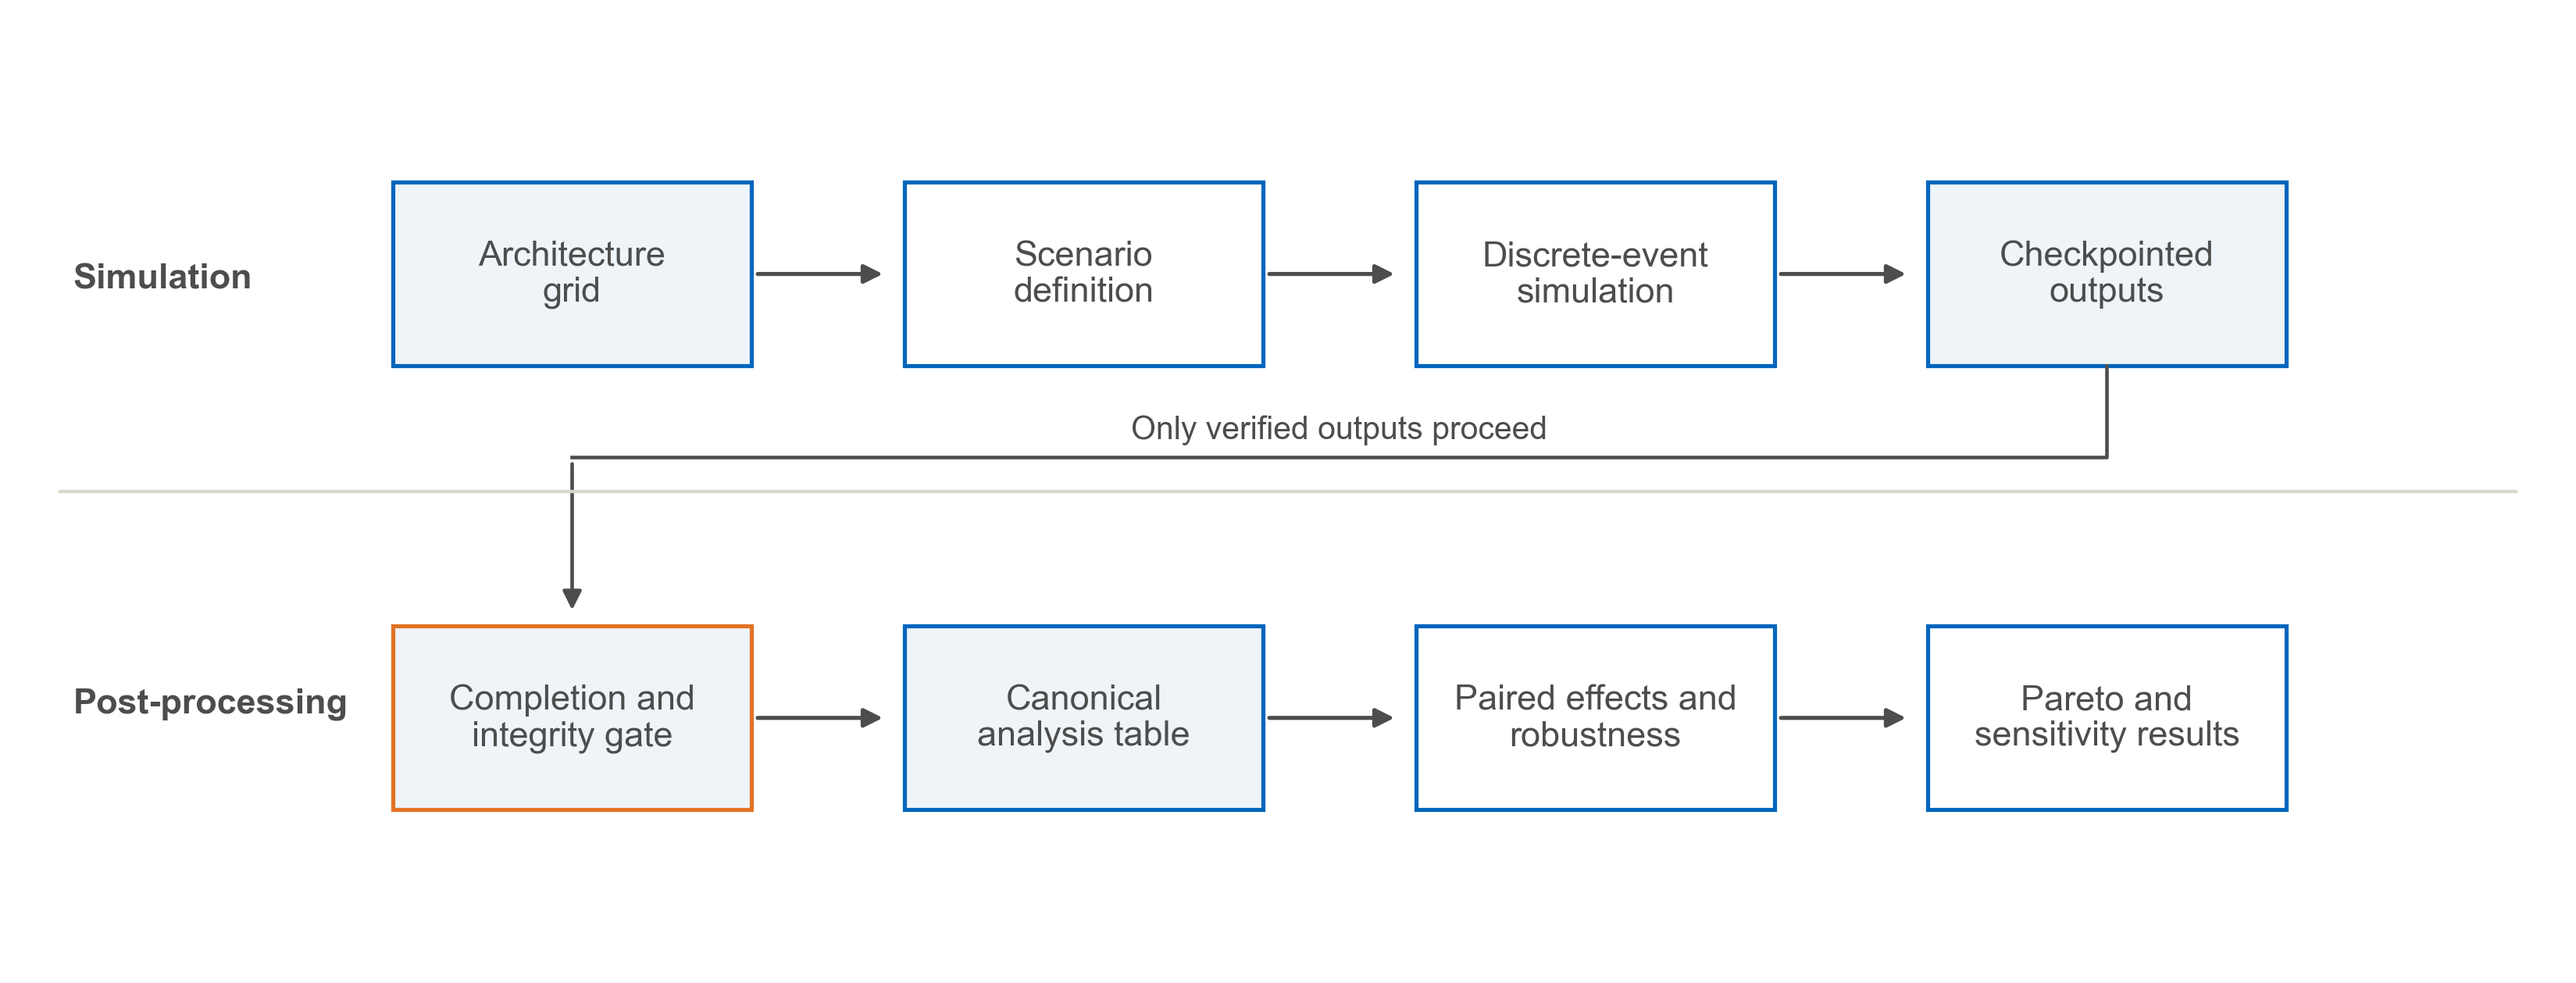
\includegraphics[width=0.96\textwidth]{figures/part1_revision/method_flow.png}
\caption{Simulation and post-processing workflow. Architectures and scenarios produce checkpointed outputs; only outputs that pass the completion and integrity gate enter the canonical analysis table, paired comparisons, robustness analysis, and Pareto evaluation.}
\label{fig:method_flow}
\end{figure}
The event order is enforced explicitly:

\begin{enumerate}
\item Freeze the regional task table and generate a Walker architecture.
\item Assign the declared fraction of central nodes with one balanced rule.
\item Propagate spacecraft states and create observation and communication windows.
\item Apply the routing-policy or failure transformation.
\item Replay transfers chronologically with packet and capacity checks.
\item Credit observation only after full task reception and before the deadline.
\item Write case-, task-, and transfer-level evidence for validation and post-processing.
\end{enumerate}
This sequence is the core method. Checkpoint file names, compression, worker memory, and restart commands are implementation details and are documented in the software appendix rather than used to explain the science.

\section{Inputs and Architecture Grid}
The simulator reads a fixed CSV rather than a live service. The task release epochs remain in UTC. Each regional run lasts at least 72 hours and extends to six hours after the latest task deadline when necessary. This produces approximately 73.1 hours for California and 73.7 hours for India.

The Walker grid varies five factors:

\begin{table}[htbp]\centering\small
\caption{Full-factorial Walker-constellation and central-node design grid.}
\label{tab:architecture_grid}
\begin{tabularx}{\textwidth}{XX}
\toprule
\textbf{Factor} & \textbf{Levels} \\
\midrule
Satellites, T & 60, 120, 180 \\
Planes, P & 3, 5, 10 \\
Altitude, H & 500, 800, 1000 km \\
Inclination, I & 60, 80, 98.6 deg \\
Central-node fraction, C & 0, 10, ..., 100 percent \\
\bottomrule
\end{tabularx}
\end{table}
Walker phasing is fixed at F = 1. The first four factors create 81 base architectures. Eleven central-node fractions per base create 891 cases per region. A case identifier such as \path{T060_P10_H0800_I0986_CN040_F1} means 60 satellites, 10 planes, 800 km altitude, 98.6 deg inclination, 40 percent central nodes, and Walker phasing 1.

The absolute number of central nodes is \texttt{N\_CN = T * C / 100}. The fraction and absolute count are both retained because CN40 represents 24 Central Nodes in a 60-satellite fleet, 48 in a 120-satellite fleet, and 72 in a 180-satellite fleet.

\begin{figure}[htbp]
\centering
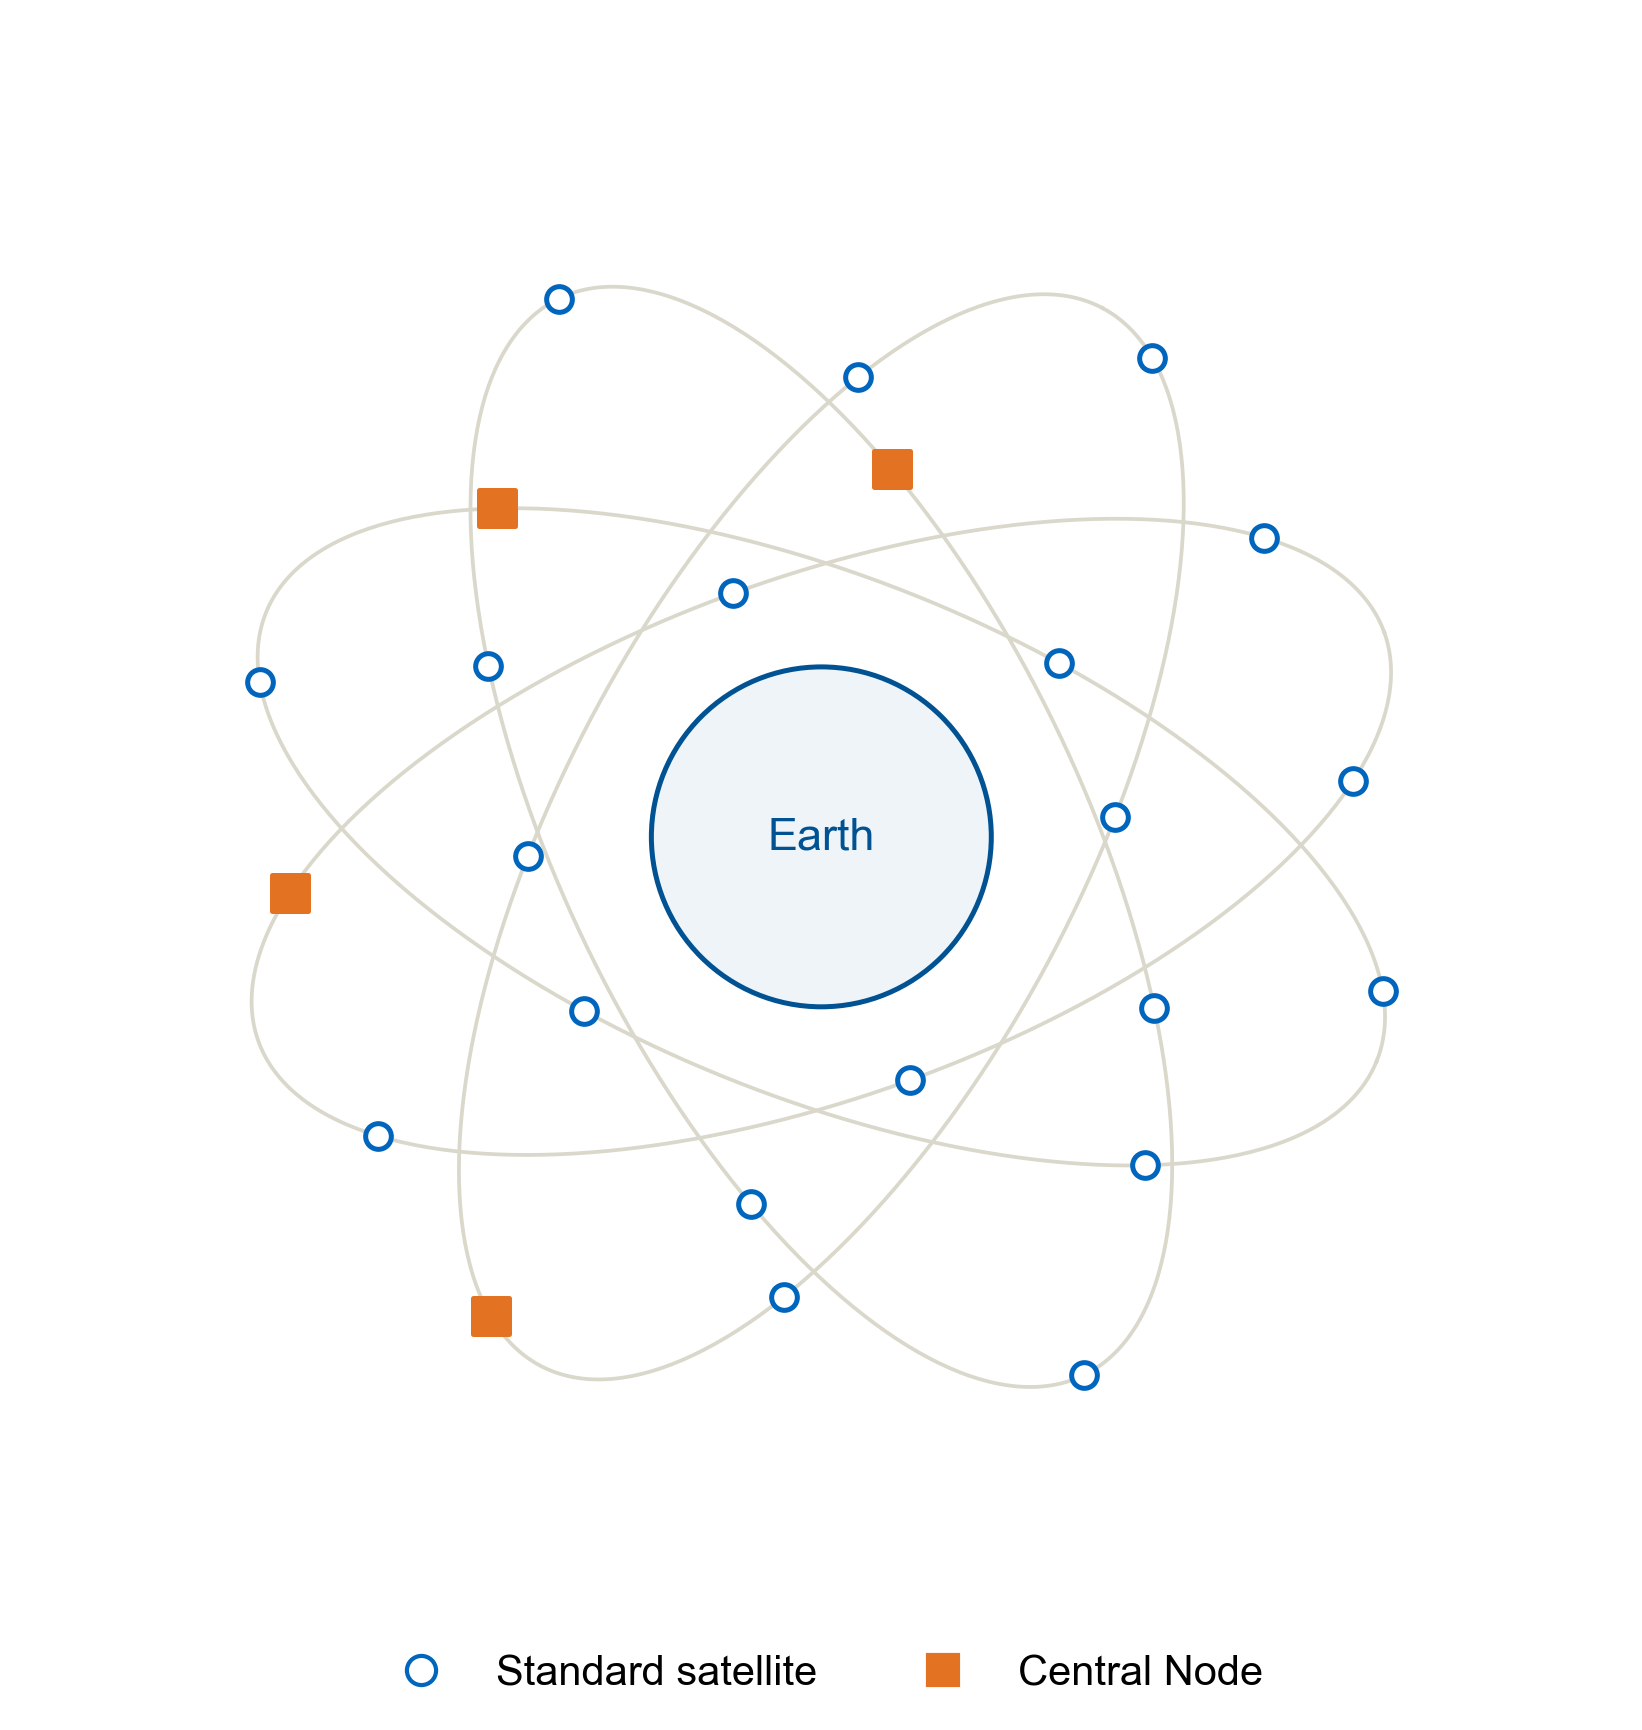
\includegraphics[width=0.96\textwidth]{figures/part1_revision/walker_cn.png}
\caption{Schematic Walker architecture with balanced central-node placement. Highlighted satellites have the routing role; all satellites keep the same orbit and sensing assumptions.}
\label{fig:walker_cn}
\end{figure}
Central nodes are spread across planes as evenly as integer constraints permit and then spaced within each plane. Fixing placement removes a manual choice from the fraction sweep. It does not establish that the placement is optimal. All nodes retain the same sensing and orbit model; only the declared routing package changes.

\section{Orbit and Observation Opportunities}
The orbital layer uses circular two-body propagation on a spherical rotating Earth within the integrated TAT-C-based workflow \citep{TATC}. The calculation uses an Earth radius of 6378.14 km, gravitational parameter 398600.44 km\textasciicircum{}3/s\textasciicircum{}2, Earth rotation rate 7.2921159e-5 rad/s, and a 60 s time step.

An observation opportunity exists when the satellite-to-task ground distance is at most 700 km. If task i is released at r\_i, has deadline d\_i, and satellite s receives it at a\_is, a valid observation is the earliest candidate access t in O\_is satisfying:

\begin{quote}\texttt{t >= max(r\_i, a\_is) and t <= d\_i.}\end{quote}
This rule prevents a pre-reception pass from being counted. The 700 km value is a mission-level access proxy, not a sensor field-of-view or pointing analysis. Cloud, smoke, illumination, slew, image quality, power, storage, and conflicts among simultaneous observations are outside the model. Results therefore remain conditional on the proxy until an observation-radius sensitivity is executed.

\section{Communication Model}
The ground segment contains one Munich station with a 10 deg minimum elevation. The active satellite-to-satellite model uses a UHF link with 2 W transmit power, 437 MHz carrier, 9.6 kHz bandwidth, and 9.6 ksymbol/s QPSK. The effective rate is limited to approximately 19.2 kbit/s; satellite-to-ground windows use 100 kbit/s.

The central-node factor is applied as a distance multiplier for each central endpoint and as the equivalent link-budget boost in the rate calculation. Under the implemented UHF parameters, the sensitivity-based upper distance is approximately 2306 km for an ordinary-to-ordinary pair, 3460 km when one endpoint is central, and 5190 km when both endpoints are central. These are eligibility ceilings, not guaranteed contacts: Earth blockage, the analytical geometry, beam angles, and the instantaneous link-rate calculation still apply.

For a window with effective rate R, usable duration delta\_t, and utilization factor eta, available capacity is:

\begin{quote}\texttt{B\_window = R * delta\_t * eta / 1e6  [Mbit].}\end{quote}
Fresh V2 uses eta = 1. A contact window records possible capacity. A transfer record proves that routing used part of that capacity. The analysis keeps the two quantities separate.

\section{Temporal Routing and Topology Policies}
\begin{figure}[htbp]
\centering
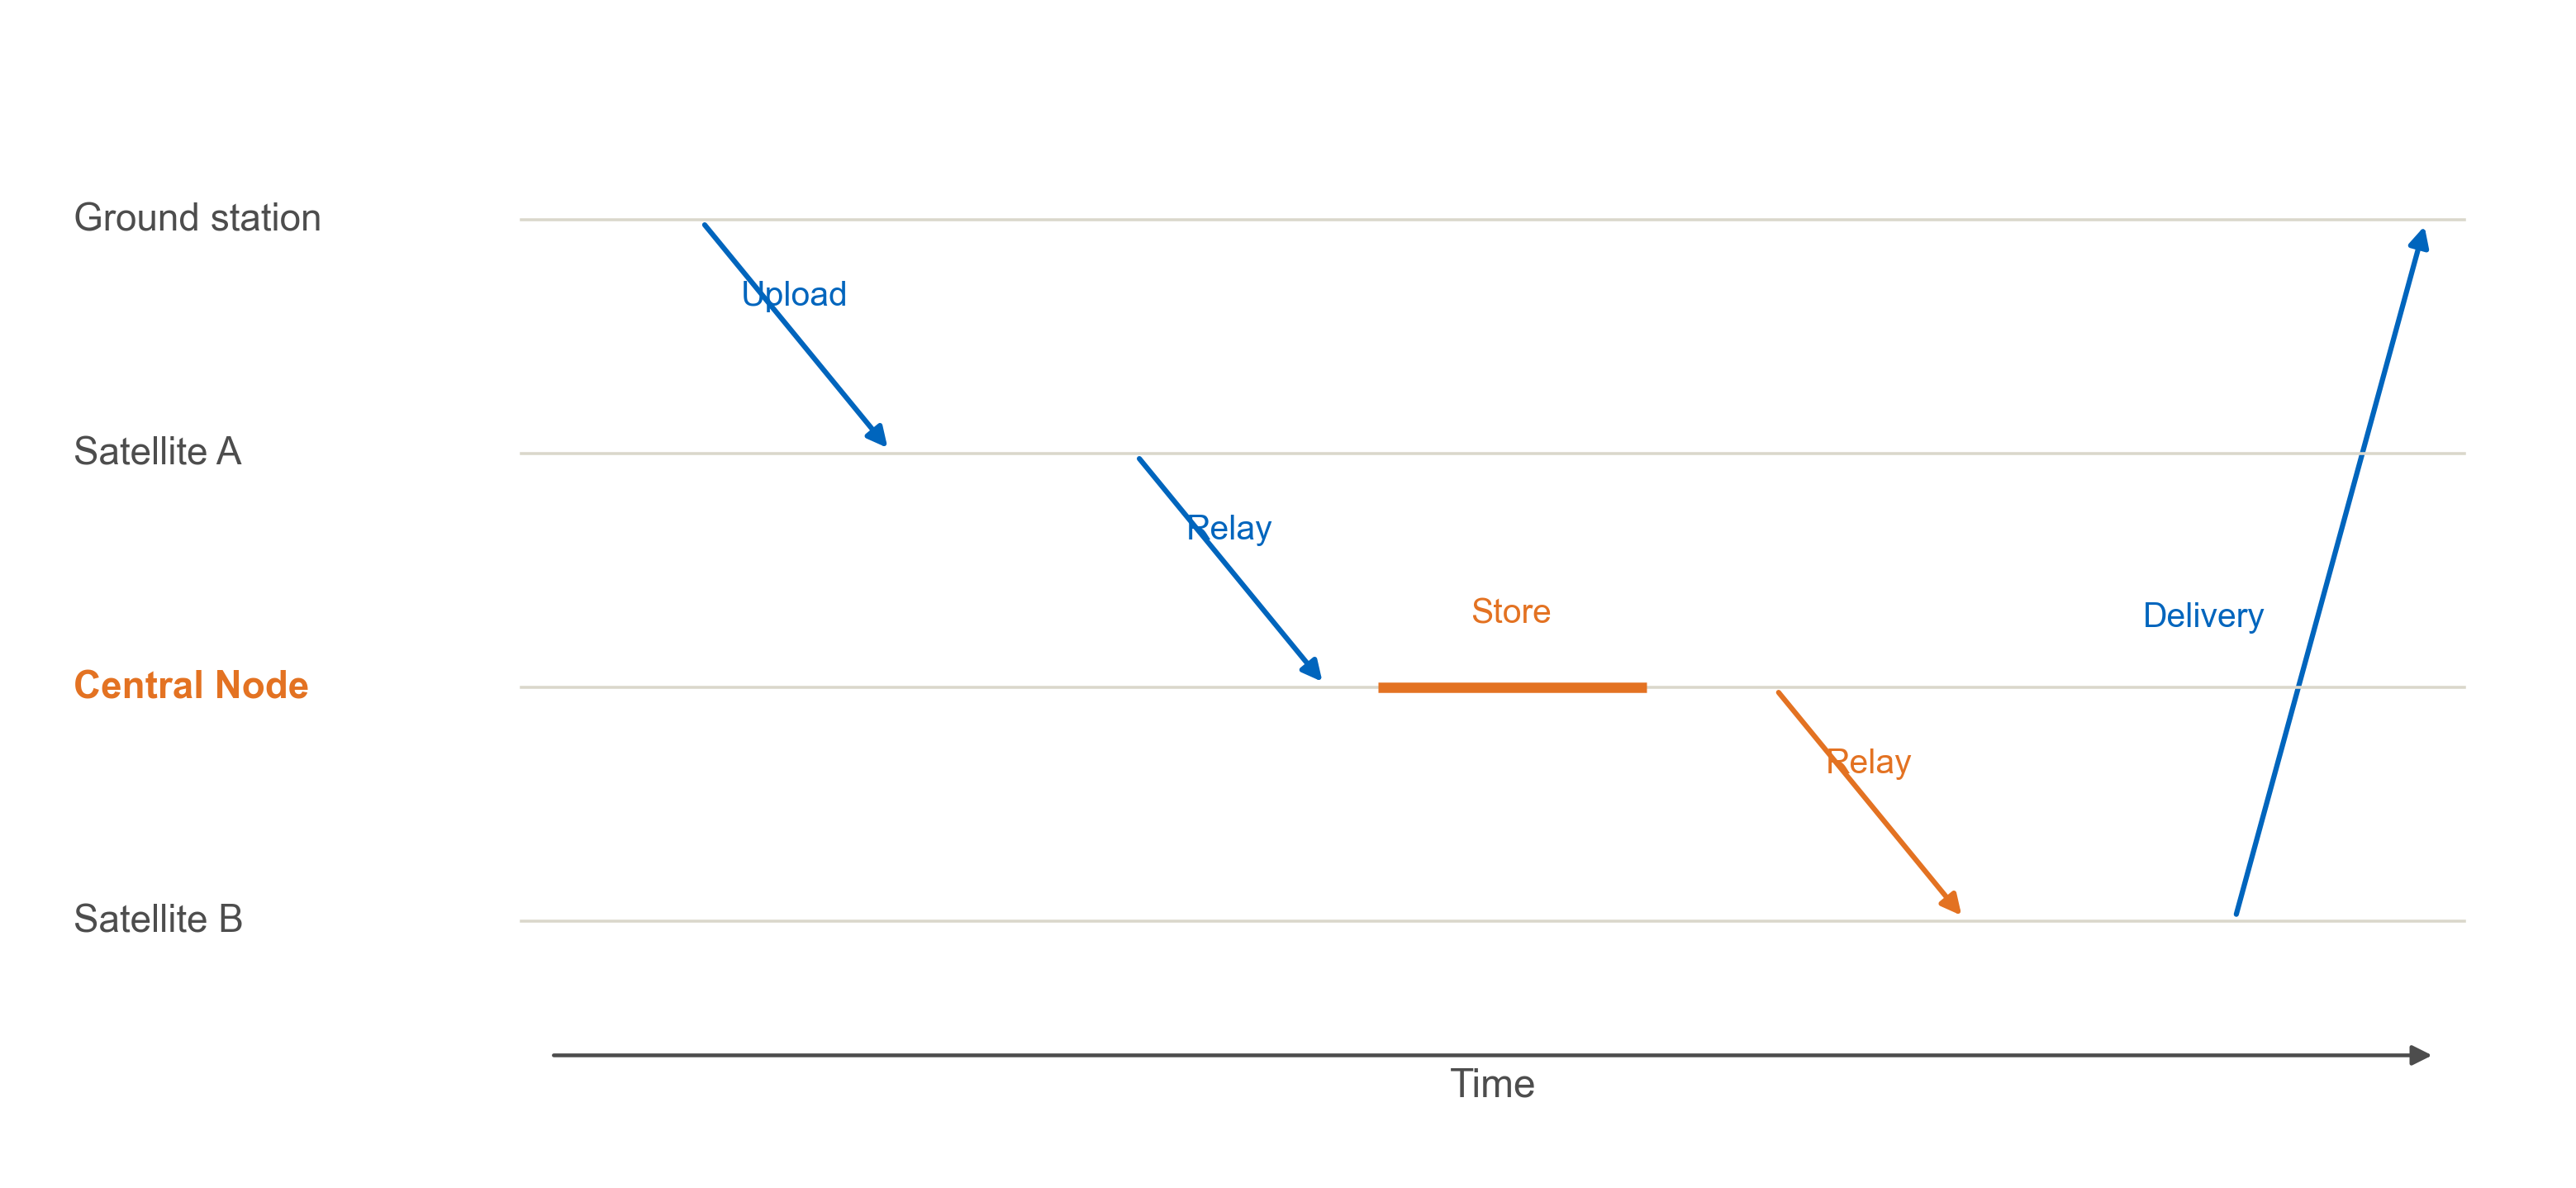
\includegraphics[width=0.96\textwidth]{figures/part1_revision/temporal_route.png}
\caption{Example temporal route. A contact is useful only if it occurs after task release and leaves the receiving satellite enough time for a later access before the deadline.}
\label{fig:temporal_route}
\end{figure}
Three topology-policy variants are replayed:

\begin{itemize}
\item \textbf{Central-only:} an inter-satellite link is usable only when at least one endpoint is central. CN0 consequently has no inter-satellite links and depends on the ground uplink. It is not a peer-to-peer baseline.
\item \textbf{Peer-only:} every feasible inter-satellite link is usable and the central label is ignored by the forwarding order.
\item \textbf{Hybrid:} every feasible link is usable, but central-node forwarding is preferred when candidates otherwise satisfy the task constraints.
\end{itemize}
At release, the task is available at the ground node. The simulator visits contact windows in chronological order. A packet is indivisible: a transfer is accepted only when the remaining window capacity can carry the complete packet. A receiver can forward only after full reception, and duplicate reception does not increase coverage.

The bounded nominal policy prioritizes deadline-relevant useful recipients and limits forwarding to three hops, three observer copies, and five central-node copies. The unlimited useful-deadline diagnostic removes those copy and hop caps while retaining the same useful-recipient and deadline definitions. It is used to show what the existing contact opportunities could support under a less restrictive forwarding rule; it is not presented as the nominal operational policy.

Routing is greedy and causal. It uses only information available at the current simulated time and does not solve a global temporal multicommodity-flow optimization. This distinction defines what conclusions can be drawn from a difference between bounded and unlimited forwarding.

\section{Scenario and Failure Transformations}
Every case is evaluated under 539 declared scenarios. The nominal case is complemented by policy, packet-size, failure, outage, degradation, and combined-stress replays. Each transformation changes one declared part of the baseline and then reruns routing and observation evaluation.

\begin{figure}[htbp]
\centering
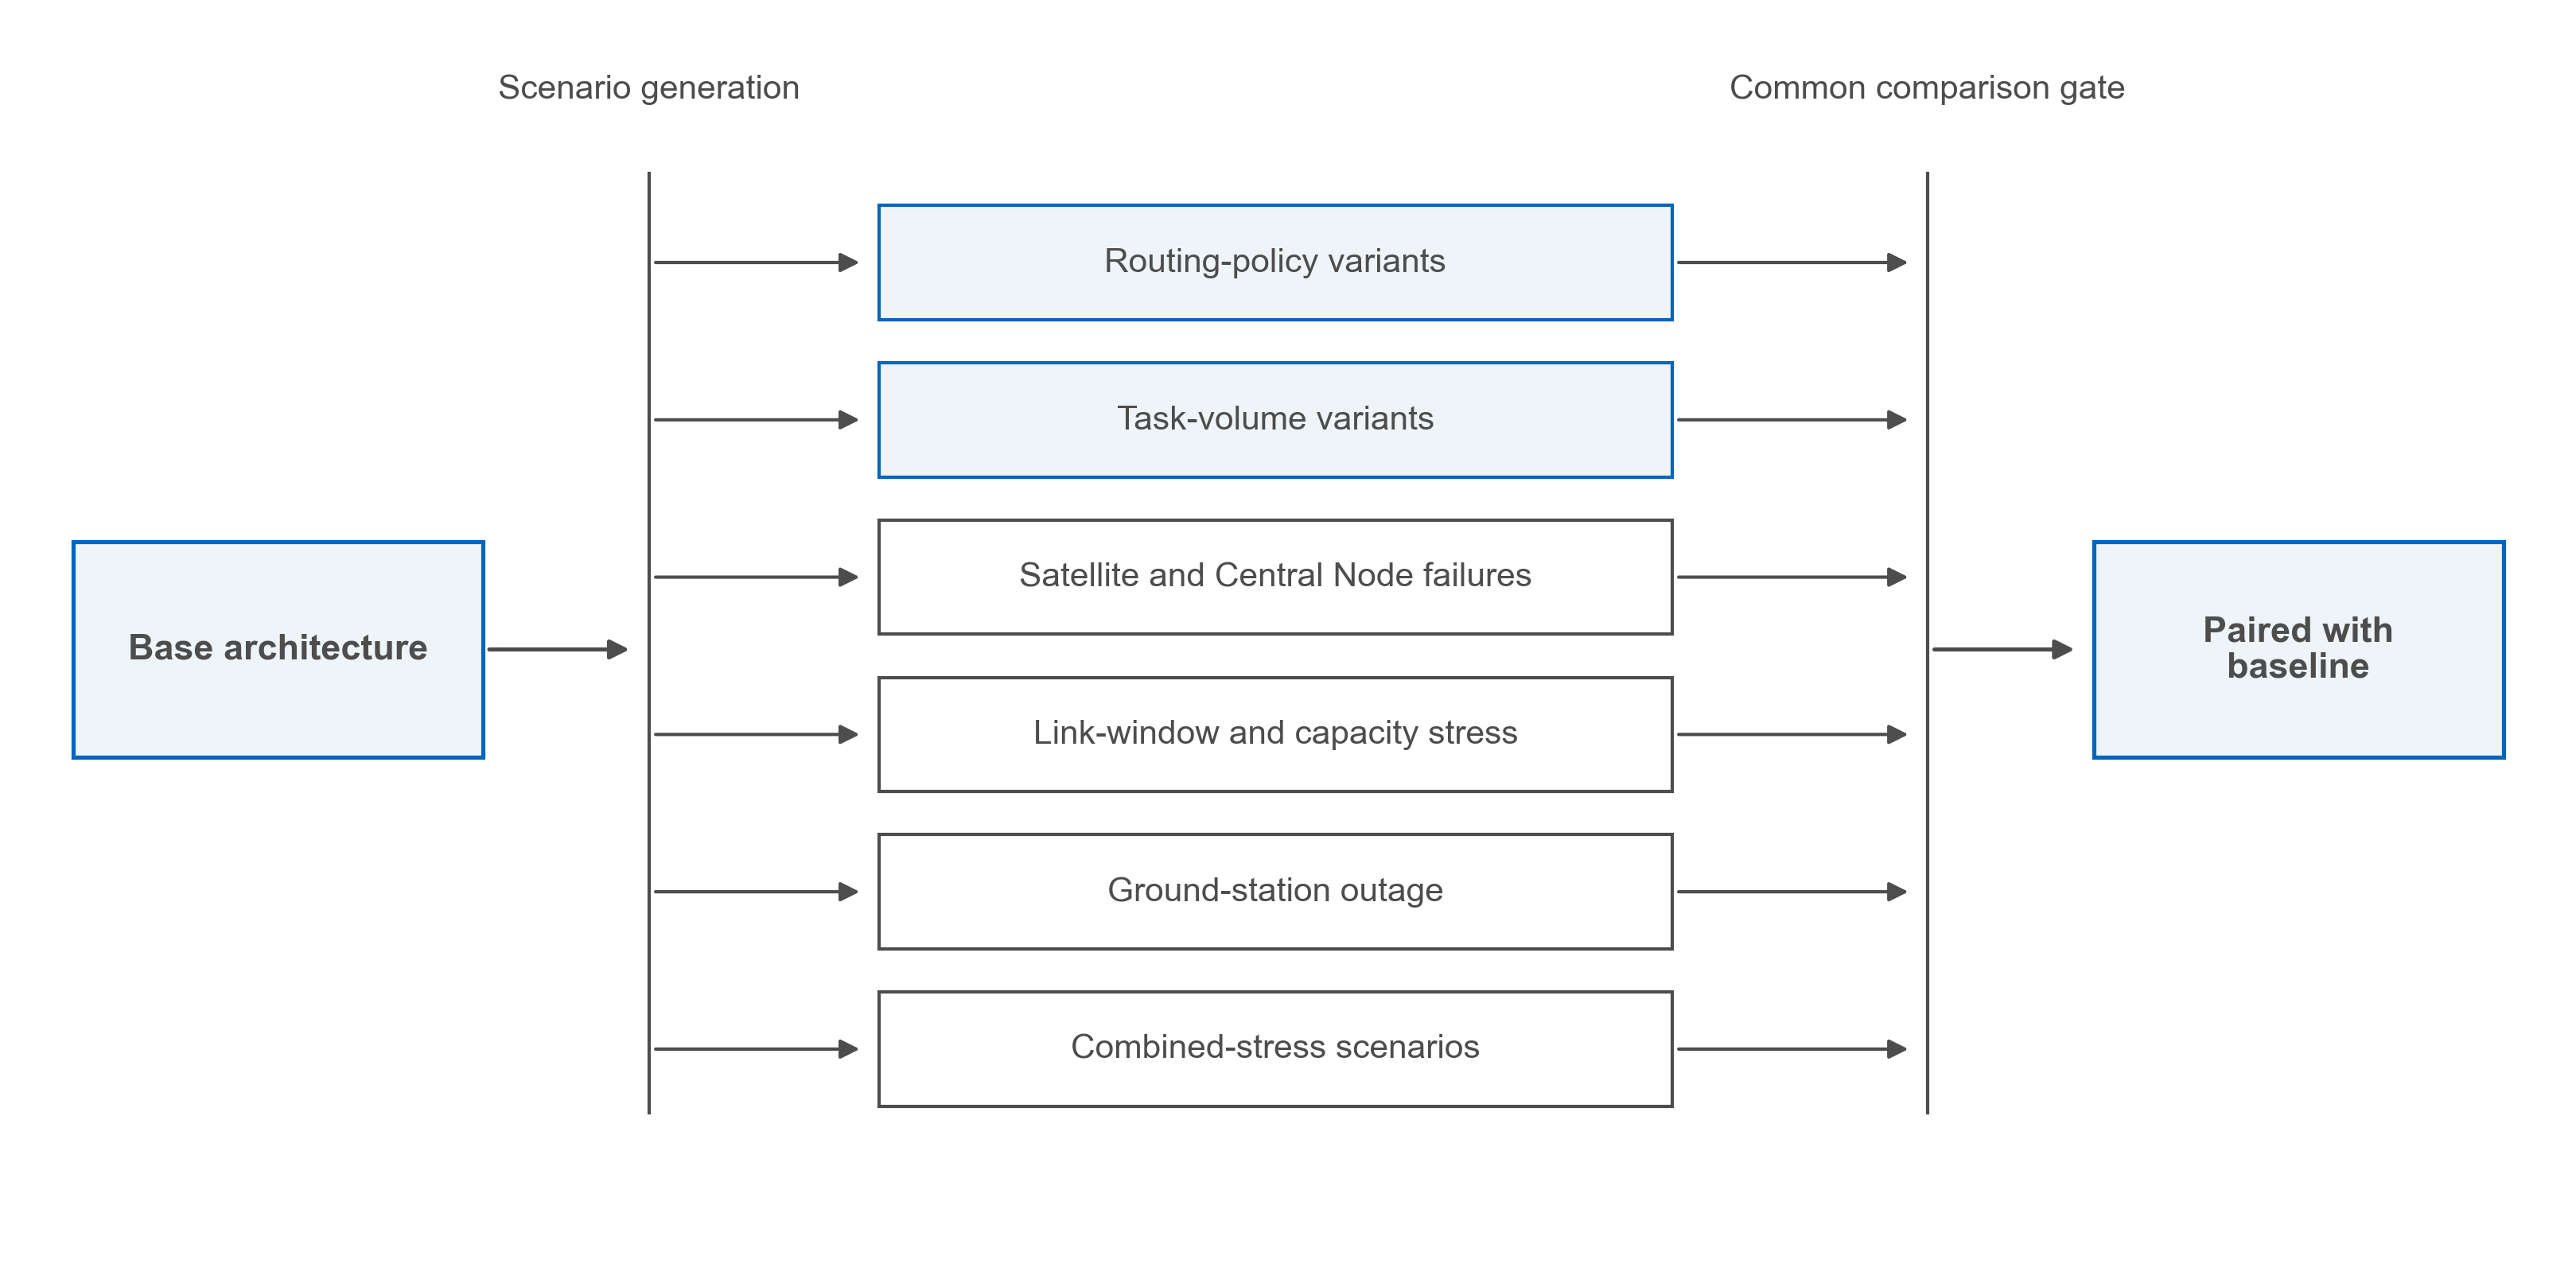
\includegraphics[width=0.96\textwidth]{figures/part1_revision/scenario_flow.png}
\caption{Scenario logic. Each policy, packet, failure, or capacity change is applied to the same baseline case before routing and observation are replayed.}
\label{fig:scenario_flow}
\end{figure}
\begin{table}[htbp]\centering\small
\caption{Scenario families and the interpretation supported by each replay.}
\label{tab:scenario_families}
\begin{tabularx}{\textwidth}{XXX}
\toprule
\textbf{Scenario family} & \textbf{Transformation} & \textbf{Question answered} \\
\midrule
Routing policy & Central-only, peer-only, hybrid, unlimited diagnostic & Is performance limited by link eligibility or forwarding bounds? \\
Packet size & 0.5x, 1x, 2x, 4x & How sensitive is the network to request volume? \\
Random satellite failure & Remove sampled satellites and their links/accesses & How much performance remains after generic node loss? \\
Random/targeted central-node failure & Remove sampled or high-importance central nodes & Is the architecture dependent on specific relays? \\
Link-window outage & Remove sampled contact windows & Is the design sensitive to lost communication opportunities? \\
Ground-station outage & Disable one sampled interval & How dependent is release and injection on the ground segment? \\
Capacity degradation & Scale window capacity & How does lower effective throughput change outcomes? \\
Combined stress & Increase packet size and remove satellites & Do load and topology damage amplify each other? \\
\bottomrule
\end{tabularx}
\end{table}
Random scenarios use deterministic seeds derived from the campaign seed, case identifier, scenario identifier, and replicate number. This makes a row reproducible and independent of worker count or completion order. Because the case identifier is part of the seed, two different architectures are not described as common-random-number pairs unless a dedicated paired-draw contract is added.

\section{Outcomes and Interpretation}
The metrics are grouped by the question they answer.

\textbf{Mission performance.} Observation fulfilment is the percentage of tasks with a valid post-reception access before deadline. Useful coverage is the average share of useful recipients reached before each task deadline. Strict completion is the share of tasks that reach every surviving useful recipient before deadline. Completion time is reported only when the required dissemination actually completes; censored tasks remain in the denominator of probability metrics.

\textbf{Communication burden.} Total transferred Mbit, transfer count, used-capacity percentage, central-node traffic share, peak node load, and the Gini coefficient of transmitted data describe how the result was achieved. A low delay obtained through much higher traffic is not treated as a free improvement.

\textbf{Robustness.} Stressed performance is compared with the same case's baseline using the raw stressed value, paired change, and retention ratio. Original and surviving denominators are stored separately so that deleting difficult recipients cannot create an artificial improvement.

\textbf{Decision support.} Exact Pareto filtering first removes cases that are no better on any declared objective and worse on at least one. Objective-weight sensitivity is then applied only to the non-redundant metric families. Rank-1 and top-5 acceptability over reproducible random weight draws describe stability under the declared preference distribution. They are not probabilities that an architecture is objectively correct.

Figure~\ref{fig:temporal_route} provides one concrete interpretation. A task can be received by Satellite A and still fail if A has no access before the deadline. It can be forwarded to Satellite B and succeed if B receives the complete packet before its later access. A figure or metric that omits this event order would answer a different question.

\section{Validation and Provenance}
No ranking is produced before the post-processing verifies inventory, schema, task provenance, declared scenario counts, duplicate keys, reconstructable metrics, and balanced comparison populations. A success marker proves structural completion only. The task hash, regional task count, and priority counts are separate scientific checks.

The audit identified an index-alignment defect in the 180-satellite India preparation. Filtering India from the combined table retained row labels 32-804. A new normalized table used labels 0-772, and pandas aligned assigned series by label rather than row position. This produced 32 invalid leading rows and excluded the final 32 Low-priority tasks from 16 April 2026. The resulting 741-task runs are internally consistent, but they are not the intended 773-task experiment.

The evidence is therefore separated:

\begin{itemize}
\item the 60- and 120-satellite California-India comparison uses the intended and matched regional inputs;
\item the 180-satellite India results are interpreted only as a within-741-task sensitivity layer; and
\item no cross-region 180-satellite effect or clean 120-to-180 scaling coefficient is claimed.
\end{itemize}
Future execution resets the regional index before normalization and binds completion records to the task-file hash, regional count, and priority distribution. This explanation preserves the usable computation without hiding the provenance limit.

\section{Reproducibility and Method Boundary}
The campaign stores scenario metrics, task metrics, selected transfer traces, central-node placement, constellation nodes, manifests, and validation records in typed Parquet files. Checkpoints make the campaign resumable, but resume behaviour is an execution feature rather than a scientific treatment. Changing worker count can change wall-clock time; it does not change the task rows, architecture identifiers, or deterministic seeds.

The method evaluates task-message dissemination and follow-up opportunity under simplified orbit, sensing, and communication assumptions. It does not model final image downlink, emergency-response action, weather, cloud, detailed pointing, energy scheduling, storage competition, lifecycle cost, or a hardware-qualified relay spacecraft. The conclusions apply to the implemented central-node routing role and the tested task populations.
